\documentclass[10pt,compress,usetitleprogressbar,aspectratio=1610,mathserif,notes]{beamer}
% Si se quita "Notes" aparece sólo la presentación, sin notas.

\usepackage[spanish, es-tabla,es-noquoting,es-noshorthands]{babel}
\usepackage{tikz}
\usepackage{listings}
\usepackage{showexpl}
\usepackage{booktabs}
\usepackage{amsthm}
\usepackage{amsmath}
\usepackage{amssymb}

% Solarized palette
\definecolor{solarizedBase03}{HTML}{002B36}
\definecolor{solarizedBase02}{HTML}{073642}
\definecolor{solarizedBase01}{HTML}{586e75}
\definecolor{solarizedBase00}{HTML}{657b83}
\definecolor{solarizedBase0}{HTML}{839496}
\definecolor{solarizedBase1}{HTML}{93a1a1}
\definecolor{solarizedBase2}{HTML}{EEE8D5}
\definecolor{solarizedBase3}{HTML}{FDF6E3}
\definecolor{solarizedYellow}{HTML}{B58900}
\definecolor{solarizedOrange}{HTML}{CB4B16}
\definecolor{solarizedRed}{HTML}{DC322F}
\definecolor{solarizedMagenta}{HTML}{D33682}
\definecolor{solarizedViolet}{HTML}{6C71C4}
\definecolor{solarizedBlue}{HTML}{268BD2}
\definecolor{solarizedCyan}{HTML}{2AA198}
\definecolor{solarizedGreen}{HTML}{859900}

\usetheme{epstfg}
\setbeamertemplate{note page}[compress]

\title{Primeros pasos en Git}
\author{Guillermo Julián Moreno \and Pedro Valero Mejía}
\date{\today}

\lstset{
  backgroundcolor=\color{solarizedBase3},
  basicstyle=\ttfamily\footnotesize\color{solarizedBase01},
  breaklines=true,
  commentstyle=\color{solarizedBase0},
  stringstyle=\color{solarizedBase1},
  keywordstyle=\color{solarizedGreen},
  language={[LaTeX]TeX},
  morekeywords={textcolor,textsubscript,subsection,subsubsection,tableofcontents,includegraphics, implies, impliedby, mathcal, mathbb},
  columns = fullflexible,
  extendedchars = true,
  literate =
    {ñ}{{\~n}}1
    {í}{{\'i}}1
    {á}{{\'a}}1
    {é}{{\'e}}1
    {ó}{{\'o}}1
}
\def\inline{\lstinline[basicstyle=\ttfamily]}

\begin{document}

\maketitle

\section{¿Qué es Git?}

\begin{frame}
\frametitle{¿Qué es?}

Es un software de control de versiones.

Básicamente permite que diversas personas trabajen de forma paralela sobre los mismos archivos evitando conflictos y pérdida de información (siempre y cuando no modifiquen exactamente la misma parte del texto)
\end{frame}


\begin{frame}
\frametitle{¿Por qué usar Git?}
\begin{enumerate}
\item Empleando dropbox, si dos compañeros nos bajamos el word del trabajo el segundo en subir sus cambios borra todo lo del primero. Git evita estos problemas.
\item Git nos permite mantener un histórico de \textbf{qué} cambios ha realizado cada persona y \textbf{cuándo}.
\item Por tanto podemos deshacer los cambios realizados en un cierto momento sin alterar el resto del proyecto.
\end{enumerate}
\end{frame}

\begin{frame}
\frametitle{¿Por qué usar Git?}

Porque a todos nos ha pasado...
\begin{figure}[b]
\centering
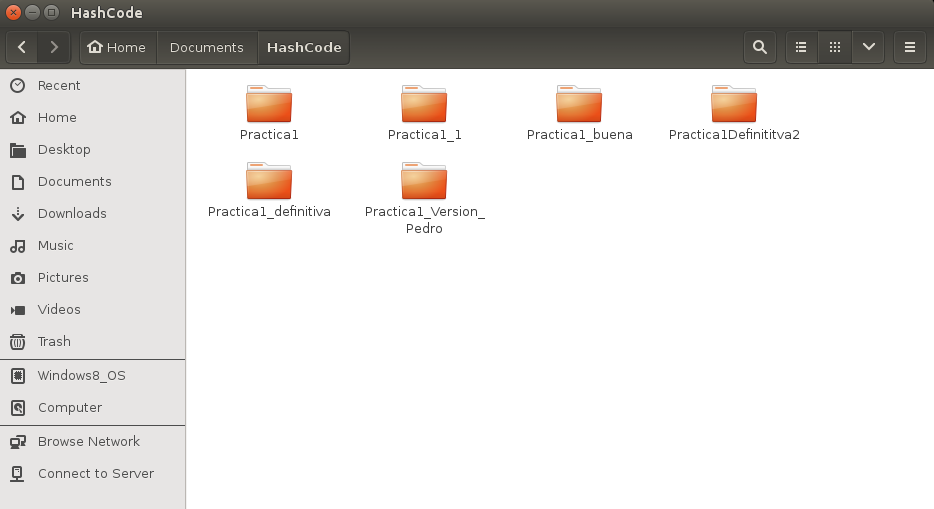
\includegraphics[height = 150pt]{dropboxClassic.png}
\end{figure}
\end{frame}

\begin{frame}
\frametitle{¿Por qué usar Git?}

Y porque a todos nos gusta ver
\begin{figure}[b]
\centering
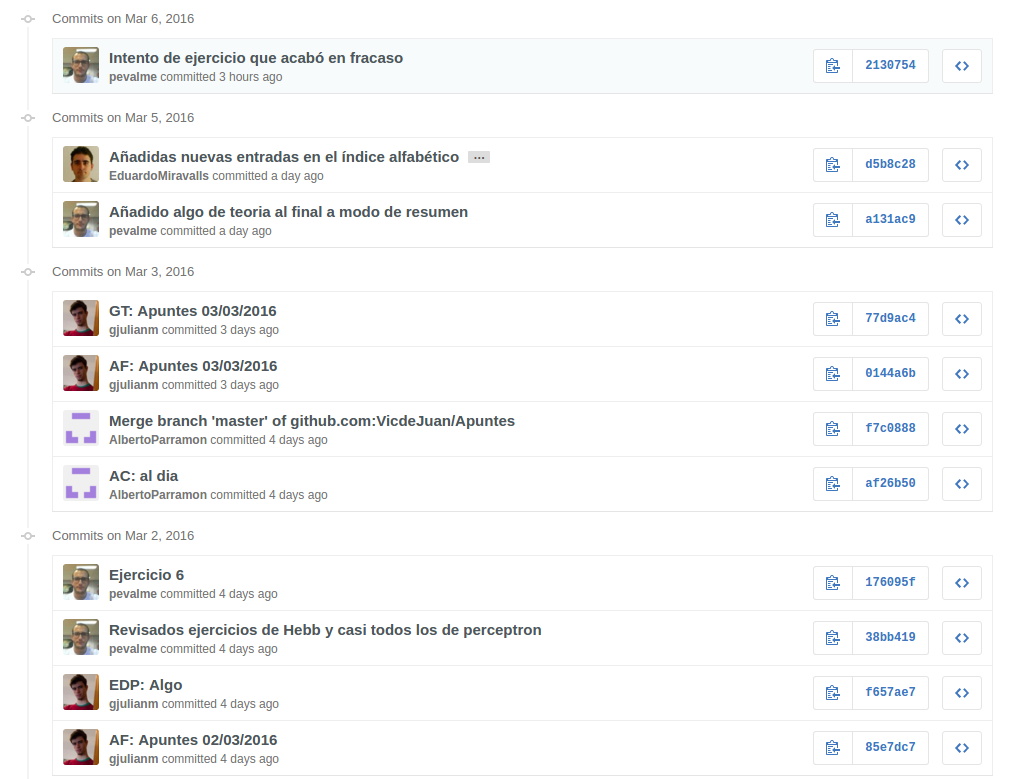
\includegraphics[height = 200pt]{gitCommits.png}
\end{figure}
\end{frame}

\section{¿Cómo funciona Git?}


\section{¿Cómo usamos Git?}


\section{Creamos un repositorio}
\end{document}
